\documentclass[a4paper,11pt]{article}
\usepackage[margin=1.5cm]{geometry}
\usepackage{amsmath,amssymb}
\usepackage{tikz}
\usepackage[dvipsnames]{xcolor}
\pagestyle{empty}

% Node styles matching the thesis conventions
\tikzset{
    dot/.style={circle, fill=black!30, draw=none, inner sep=0.5pt},
    bigdot/.style={circle, fill=black, draw=none, inner sep=3pt},
    bluedot/.style={circle, fill=blue, draw=none, inner sep=2pt},
    reddot/.style={circle, fill=red, draw=none, inner sep=2pt},
    % Highlighted face labels (colored background)
    hlpink/.style={fill=pink, rounded corners=2pt, inner sep=1pt},
    hlblue/.style={fill=blue!20, rounded corners=2pt, inner sep=1pt},
    hlred/.style={fill=red!25, rounded corners=2pt, inner sep=1pt},
    hlyellow/.style={fill=yellow!50, rounded corners=2pt, inner sep=1pt},
    hlorange/.style={fill=orange!40, rounded corners=2pt, inner sep=1pt},
    hlpurple/.style={fill=purple!25, rounded corners=2pt, inner sep=1pt},
}

\begin{document}

% ============================================================
% DIAGRAM 1: Fomin's Local Rules (single face)
% ============================================================
\begin{tikzpicture}[scale=1.8]
\node at (2,2) {$\color{blue}x$};
\node at (2.5,2.5) {$\color{blue}\nu$};
\node at (2.5,1.5) {$\color{red}\lambda$};
\node at (1.5,2.5) {$\color{blue}\rho$};
\node at (1.5,1.5) {$\color{blue}\mu$};
\end{tikzpicture}

% ============================================================
% DIAGRAM 2: Complete Fomin Growth Diagram
% ============================================================
% Permutation σ = [5,3,6,1,4,7,2]
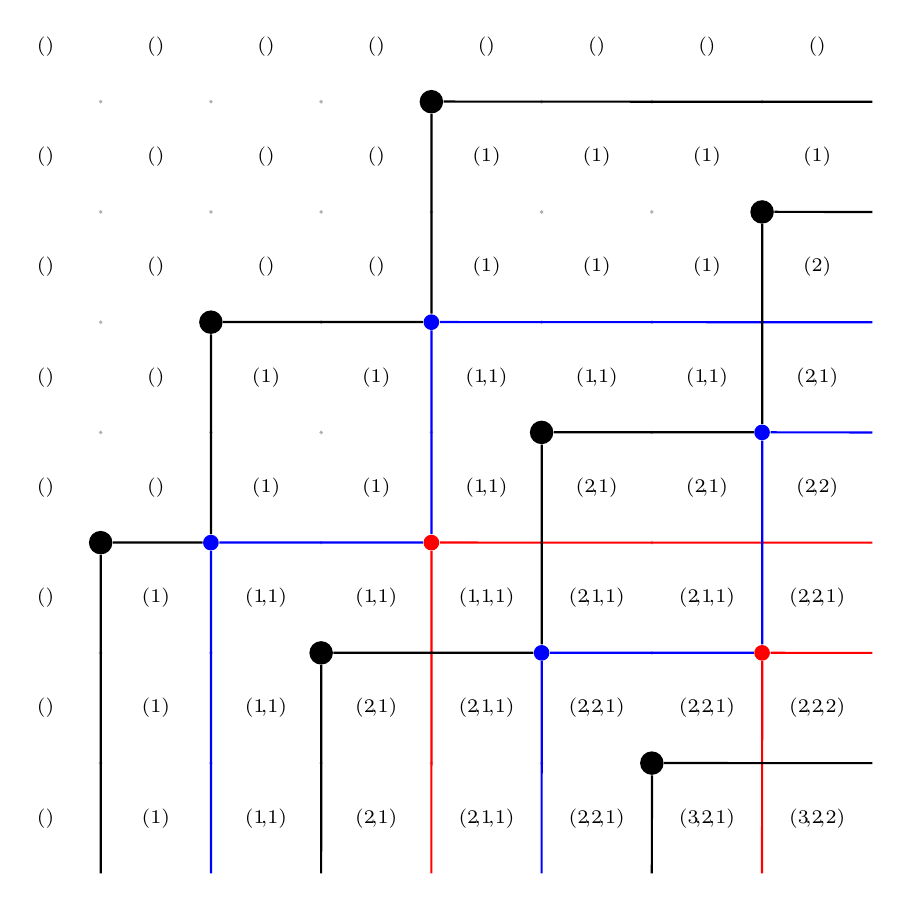
\begin{tikzpicture}[scale=1.4]

% Background grid
\foreach \x in {1,...,7}
  \foreach \y in {1,...,7}
    \node[dot] at (\x,\y) {};

% === Partition labels in faces ===
% Left column
\foreach \y in {0.5,1.5,...,7.5}
  \node at (0.5,\y) {\scriptsize$()$};
% Top row
\foreach \x in {1.5,2.5,...,7.5}
  \node at (\x,7.5) {\scriptsize$()$};

% Row y=6.5
\node at (1.5,6.5) {\scriptsize$()$};
\node at (2.5,6.5) {\scriptsize$()$};
\node at (3.5,6.5) {\scriptsize$()$};
\node at (4.5,6.5) {\scriptsize$(1)$};
\node at (5.5,6.5) {\scriptsize$(1)$};
\node at (6.5,6.5) {\scriptsize$(1)$};
\node at (7.5,6.5) {\scriptsize$(1)$};

% Row y=5.5
\node at (1.5,5.5) {\scriptsize$()$};
\node at (2.5,5.5) {\scriptsize$()$};
\node at (3.5,5.5) {\scriptsize$()$};
\node at (4.5,5.5) {\scriptsize$(1)$};
\node at (5.5,5.5) {\scriptsize$(1)$};
\node at (6.5,5.5) {\scriptsize$(1)$};
\node at (7.5,5.5) {\scriptsize$(2)$};

% Row y=4.5
\node at (1.5,4.5) {\scriptsize$()$};
\node at (2.5,4.5) {\scriptsize$(1)$};
\node at (3.5,4.5) {\scriptsize$(1)$};
\node at (4.5,4.5) {\scriptsize$(1\!,\!1)$};
\node at (5.5,4.5) {\scriptsize$(1\!,\!1)$};
\node at (6.5,4.5) {\scriptsize$(1\!,\!1)$};
\node at (7.5,4.5) {\scriptsize$(2\!,\!1)$};

% Row y=3.5
\node at (1.5,3.5) {\scriptsize$()$};
\node at (2.5,3.5) {\scriptsize$(1)$};
\node at (3.5,3.5) {\scriptsize$(1)$};
\node at (4.5,3.5) {\scriptsize$(1\!,\!1)$};
\node at (5.5,3.5) {\scriptsize$(2\!,\!1)$};
\node at (6.5,3.5) {\scriptsize$(2\!,\!1)$};
\node at (7.5,3.5) {\scriptsize$(2\!,\!2)$};

% Row y=2.5
\node at (1.5,2.5) {\scriptsize$(1)$};
\node at (2.5,2.5) {\scriptsize$(1\!,\!1)$};
\node at (3.5,2.5) {\scriptsize$(1\!,\!1)$};
\node at (4.5,2.5) {\scriptsize$(1\!,\!1\!,\!1)$};
\node at (5.5,2.5) {\scriptsize$(2\!,\!1\!,\!1)$};
\node at (6.5,2.5) {\scriptsize$(2\!,\!1\!,\!1)$};
\node at (7.5,2.5) {\scriptsize$(2\!,\!2\!,\!1)$};

% Row y=1.5
\node at (1.5,1.5) {\scriptsize$(1)$};
\node at (2.5,1.5) {\scriptsize$(1\!,\!1)$};
\node at (3.5,1.5) {\scriptsize$(2\!,\!1)$};
\node at (4.5,1.5) {\scriptsize$(2\!,\!1\!,\!1)$};
\node at (5.5,1.5) {\scriptsize$(2\!,\!2\!,\!1)$};
\node at (6.5,1.5) {\scriptsize$(2\!,\!2\!,\!1)$};
\node at (7.5,1.5) {\scriptsize$(2\!,\!2\!,\!2)$};

% Row y=0.5
\node at (1.5,0.5) {\scriptsize$(1)$};
\node at (2.5,0.5) {\scriptsize$(1\!,\!1)$};
\node at (3.5,0.5) {\scriptsize$(2\!,\!1)$};
\node at (4.5,0.5) {\scriptsize$(2\!,\!1\!,\!1)$};
\node at (5.5,0.5) {\scriptsize$(2\!,\!2\!,\!1)$};
\node at (6.5,0.5) {\scriptsize$(3\!,\!2\!,\!1)$};
\node at (7.5,0.5) {\scriptsize$(3\!,\!2\!,\!2)$};

% === Permutation dots and shadow lines ===
% First decreasing subsequence: (1,5),(2,3),(4,1) -> cols 1,2,4 rows 5,3,1
% Mapped to grid: (col, row_from_bottom) but thesis uses (col, sigma(col))
% sigma = [5,3,6,1,4,7,2]
% Black dots at permutation entries
\node[bigdot] (B1) at (1,3) {};   % really sigma uses different coords
\node[bigdot] (B2) at (2,5) {};
\node[bigdot] (B3) at (4,7) {};
\node[bluedot] (Bl1) at (2,3) {};
\node[bluedot] (Bl2) at (4,5) {};
\node[reddot] (R1) at (4,3) {};

\node[bigdot] (B4) at (3,2) {};
\node[bigdot] (B5) at (5,4) {};
\node[bigdot] (B6) at (7,6) {};
\node[bluedot] (Bl3) at (5,2) {};
\node[bluedot] (Bl4) at (7,4) {};
\node[reddot] (R2) at (7,2) {};

\node[bigdot] (B7) at (6,1) {};

% Shadow lines - first group
\draw[black, thick] (1,0) -- (B1) -- (Bl1) -- (B2) -- (Bl2) -- (B3) -- (8,7);
\draw[blue, thick]  (2,0) -- (Bl1) -- (R1) -- (Bl2) -- (8,5);
\draw[red, thick]   (4,0) -- (R1) -- (8,3);
% Second group
\draw[black, thick] (3,0) -- (B4) -- (Bl3) -- (B5) -- (Bl4) -- (B6) -- (8,6);
\draw[blue, thick]  (5,0) -- (Bl3) -- (R2) -- (Bl4) -- (8,4);
\draw[red, thick]   (7,0) -- (R2) -- (8,2);
% Third group
\draw[black, thick] (6,0) -- (B7) -- (8,1);

\end{tikzpicture}

% ============================================================
% DIAGRAM 3: Local Rules Example (color-coded faces)
% ============================================================
%   Yellow = Rule 1 (x=1, μ=ν=ρ, add box to first row)
%   Blue   = Rule 2 (x=0, μ=ν=ρ, λ=ρ)
%   Red    = Rule 3 (x=0, μ=ρ≠ν, vertical shadow)
%   Pink   = Rule 4 (x=0, ν=ρ≠μ, horizontal shadow)
%   Orange = Rule 5 (x=0, μ,ν,ρ pairwise distinct, λ=μ∪ν)
%   Purple = Rule 6 (x=0, μ=ν≠ρ, bounce to next row)
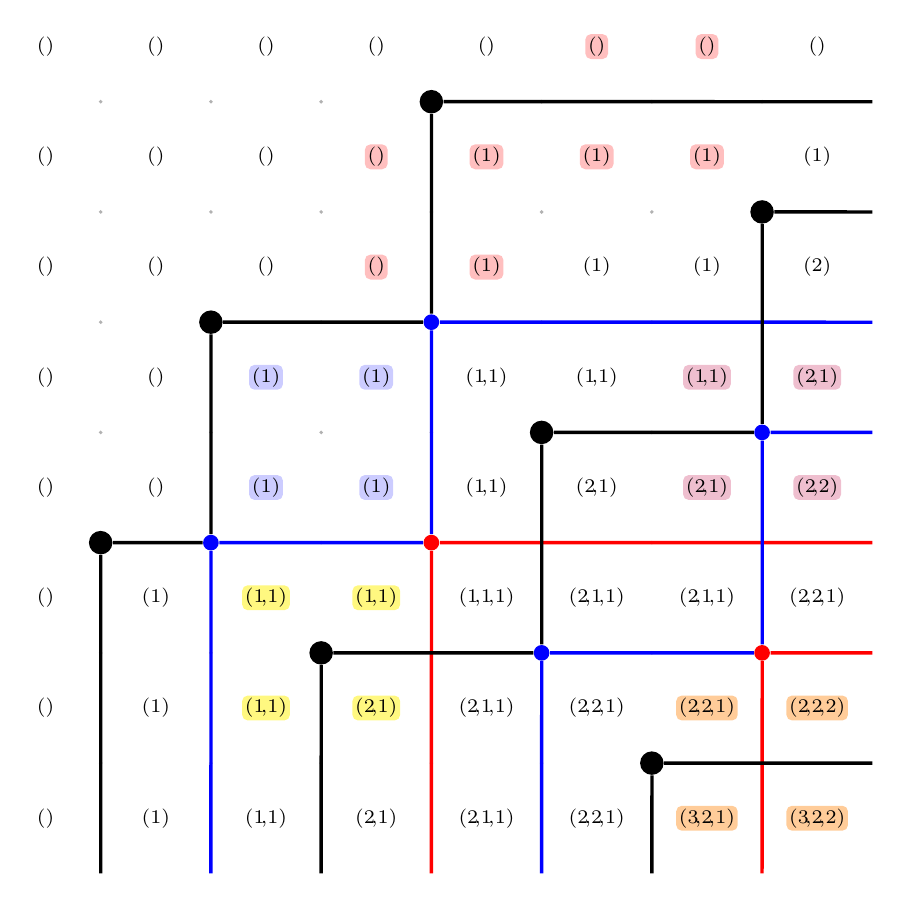
\begin{tikzpicture}[scale=1.4]

% Background grid
\foreach \x in {1,...,7}
  \foreach \y in {1,...,7}
    \node[dot] at (\x,\y) {};

% Left column
\foreach \y in {0.5,1.5,...,7.5}
  \node at (0.5,\y) {\scriptsize$()$};

% Top row (y=7.5) - pink highlights for Rule 4
\node at (1.5,7.5) {\scriptsize$()$};
\node at (2.5,7.5) {\scriptsize$()$};
\node at (3.5,7.5) {\scriptsize$()$};
\node at (4.5,7.5) {\scriptsize$()$};
\node[hlpink] at (5.5,7.5) {\scriptsize$()$};
\node[hlpink] at (6.5,7.5) {\scriptsize$()$};
\node at (7.5,7.5) {\scriptsize$()$};

% Row y=6.5 - red for Rule 3, pink for Rule 4
\node at (1.5,6.5) {\scriptsize$()$};
\node at (2.5,6.5) {\scriptsize$()$};
\node[hlred] at (3.5,6.5) {\scriptsize$()$};
\node[hlred] at (4.5,6.5) {\scriptsize$(1)$};
\node[hlpink] at (5.5,6.5) {\scriptsize$(1)$};
\node[hlpink] at (6.5,6.5) {\scriptsize$(1)$};
\node at (7.5,6.5) {\scriptsize$(1)$};

% Row y=5.5 - red for Rule 3
\node at (1.5,5.5) {\scriptsize$()$};
\node at (2.5,5.5) {\scriptsize$()$};
\node[hlred] at (3.5,5.5) {\scriptsize$()$};
\node[hlred] at (4.5,5.5) {\scriptsize$(1)$};
\node at (5.5,5.5) {\scriptsize$(1)$};
\node at (6.5,5.5) {\scriptsize$(1)$};
\node at (7.5,5.5) {\scriptsize$(2)$};

% Row y=4.5 - blue for Rule 2, purple for Rule 6
\node at (1.5,4.5) {\scriptsize$()$};
\node[hlblue] at (2.5,4.5) {\scriptsize$(1)$};
\node[hlblue] at (3.5,4.5) {\scriptsize$(1)$};
\node at (4.5,4.5) {\scriptsize$(1\!,\!1)$};
\node at (5.5,4.5) {\scriptsize$(1\!,\!1)$};
\node[hlpurple] at (6.5,4.5) {\scriptsize$(1\!,\!1)$};
\node[hlpurple] at (7.5,4.5) {\scriptsize$(2\!,\!1)$};

% Row y=3.5 - blue for Rule 2, purple for Rule 6
\node at (1.5,3.5) {\scriptsize$()$};
\node[hlblue] at (2.5,3.5) {\scriptsize$(1)$};
\node[hlblue] at (3.5,3.5) {\scriptsize$(1)$};
\node at (4.5,3.5) {\scriptsize$(1\!,\!1)$};
\node at (5.5,3.5) {\scriptsize$(2\!,\!1)$};
\node[hlpurple] at (6.5,3.5) {\scriptsize$(2\!,\!1)$};
\node[hlpurple] at (7.5,3.5) {\scriptsize$(2\!,\!2)$};

% Row y=2.5 - yellow for Rule 1
\node at (1.5,2.5) {\scriptsize$(1)$};
\node[hlyellow] at (2.5,2.5) {\scriptsize$(1\!,\!1)$};
\node[hlyellow] at (3.5,2.5) {\scriptsize$(1\!,\!1)$};
\node at (4.5,2.5) {\scriptsize$(1\!,\!1\!,\!1)$};
\node at (5.5,2.5) {\scriptsize$(2\!,\!1\!,\!1)$};
\node at (6.5,2.5) {\scriptsize$(2\!,\!1\!,\!1)$};
\node at (7.5,2.5) {\scriptsize$(2\!,\!2\!,\!1)$};

% Row y=1.5 - yellow for Rule 1, orange for Rule 5
\node at (1.5,1.5) {\scriptsize$(1)$};
\node[hlyellow] at (2.5,1.5) {\scriptsize$(1\!,\!1)$};
\node[hlyellow] at (3.5,1.5) {\scriptsize$(2\!,\!1)$};
\node at (4.5,1.5) {\scriptsize$(2\!,\!1\!,\!1)$};
\node at (5.5,1.5) {\scriptsize$(2\!,\!2\!,\!1)$};
\node[hlorange] at (6.5,1.5) {\scriptsize$(2\!,\!2\!,\!1)$};
\node[hlorange] at (7.5,1.5) {\scriptsize$(2\!,\!2\!,\!2)$};

% Row y=0.5 - orange for Rule 5
\node at (1.5,0.5) {\scriptsize$(1)$};
\node at (2.5,0.5) {\scriptsize$(1\!,\!1)$};
\node at (3.5,0.5) {\scriptsize$(2\!,\!1)$};
\node at (4.5,0.5) {\scriptsize$(2\!,\!1\!,\!1)$};
\node at (5.5,0.5) {\scriptsize$(2\!,\!2\!,\!1)$};
\node[hlorange] at (6.5,0.5) {\scriptsize$(3\!,\!2\!,\!1)$};
\node[hlorange] at (7.5,0.5) {\scriptsize$(3\!,\!2\!,\!2)$};

% Shadow lines and dots
\node[bigdot] (B1) at (1,3) {};
\node[bigdot] (B2) at (2,5) {};
\node[bigdot] (B3) at (4,7) {};
\node[bluedot] (Bl1) at (2,3) {};
\node[bluedot] (Bl2) at (4,5) {};
\node[reddot] (R1) at (4,3) {};

\node[bigdot] (B4) at (3,2) {};
\node[bigdot] (B5) at (5,4) {};
\node[bigdot] (B6) at (7,6) {};
\node[bluedot] (Bl3) at (5,2) {};
\node[bluedot] (Bl4) at (7,4) {};
\node[reddot] (R2) at (7,2) {};

\node[bigdot] (B7) at (6,1) {};

\draw[black, very thick] (1,0) -- (B1) -- (Bl1) -- (B2) -- (Bl2) -- (B3) -- (8,7);
\draw[blue, very thick]  (2,0) -- (Bl1) -- (R1) -- (Bl2) -- (8,5);
\draw[red, very thick]   (4,0) -- (R1) -- (8,3);

\draw[black, very thick] (3,0) -- (B4) -- (Bl3) -- (B5) -- (Bl4) -- (B6) -- (8,6);
\draw[blue, very thick]  (5,0) -- (Bl3) -- (R2) -- (Bl4) -- (8,4);
\draw[red, very thick]   (7,0) -- (R2) -- (8,2);

\draw[black, very thick] (6,0) -- (B7) -- (8,1);

\end{tikzpicture}

% ============================================================
% DIAGRAM 4: Cylindric Growth Diagram (π = 00101)
% ============================================================
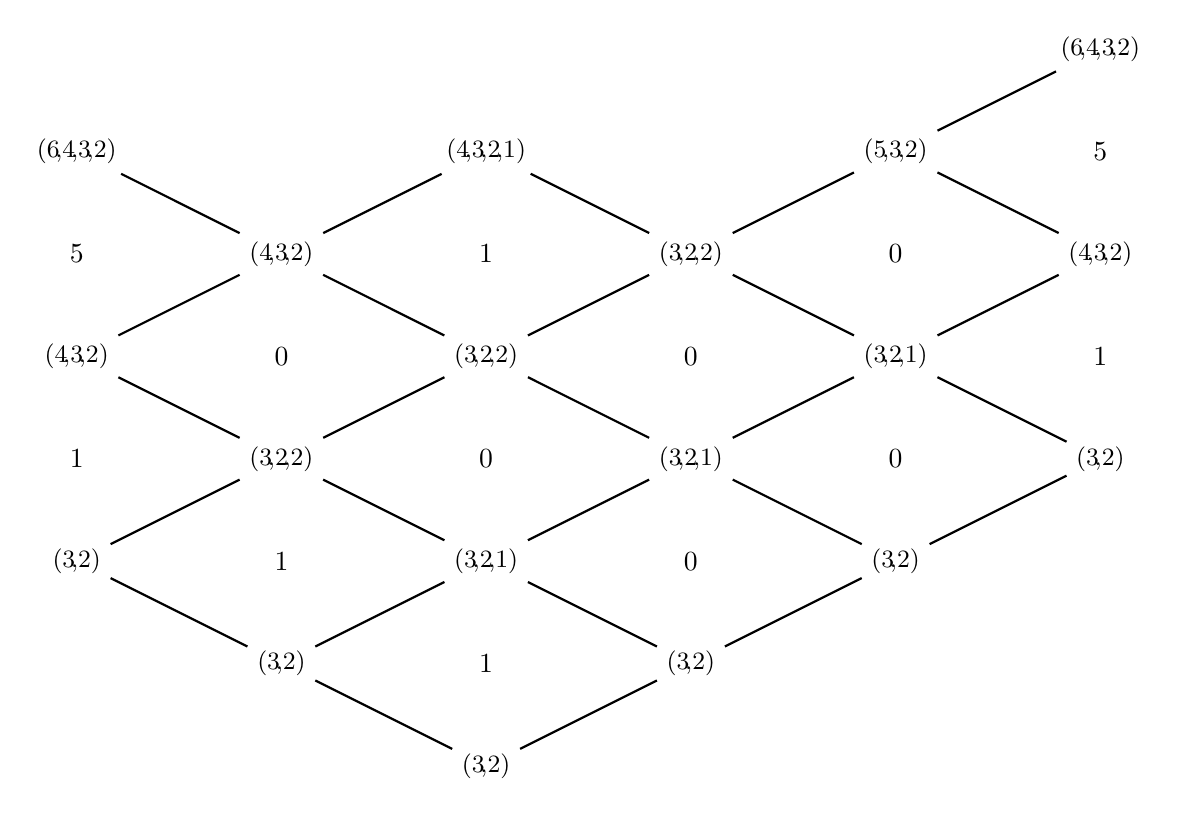
\begin{tikzpicture}[scale=1.3]

% === Vertices (bottom row -- all labelled γ = (3,2)) ===
\node (A0) at (-4,2)  {\small$(3\!,\!2)$};
\node (B0) at (-2,1)  {\small$(3\!,\!2)$};
\node (C0) at (0,0)   {\small$(3\!,\!2)$};
\node (D0) at (2,1)   {\small$(3\!,\!2)$};
\node (E0) at (4,2)   {\small$(3\!,\!2)$};
\node (F0) at (6,3)   {\small$(3\!,\!2)$};

% === Vertices (depth 1) ===
\node (A1) at (-4,4)  {\small$(4\!,\!3\!,\!2)$};
\node (B1) at (-2,3)  {\small$(3\!,\!2\!,\!2)$};
\node (C1) at (0,2)   {\small$(3\!,\!2\!,\!1)$};
\node (D1) at (2,3)   {\small$(3\!,\!2\!,\!1)$};
\node (E1) at (4,4)   {\small$(3\!,\!2\!,\!1)$};
\node (F1) at (6,5)   {\small$(4\!,\!3\!,\!2)$};

% === Vertices (depth 2) ===
\node (A2) at (-4,6)  {\small$(6\!,\!4\!,\!3\!,\!2)$};
\node (B2) at (-2,5)  {\small$(4\!,\!3\!,\!2)$};
\node (C2) at (0,4)   {\small$(3\!,\!2\!,\!2)$};
\node (D2) at (2,5)   {\small$(3\!,\!2\!,\!2)$};
\node (E2) at (4,6)   {\small$(5\!,\!3\!,\!2)$};
\node (F2) at (6,7)   {\small$(6\!,\!4\!,\!3\!,\!2)$};

% === Top vertex (depth 3) ===
\node (C3) at (0,6)   {\small$(4\!,\!3\!,\!2\!,\!1)$};

% === Horizontal edges ===
\draw[thick] (A0) -- (B0) -- (C0) -- (D0) -- (E0) -- (F0);
\draw[thick] (A1) -- (B1) -- (C1) -- (D1) -- (E1) -- (F1);
\draw[thick] (A2) -- (B2) -- (C2) -- (D2) -- (E2) -- (F2);

% === Diagonal edges ===
% SW diagonals (π_k = 0)
\draw[thick] (A0) -- (B1) -- (C2);
\draw[thick] (B0) -- (C1);
\draw[thick] (A1) -- (B2) -- (C3);
% NW diagonals (π_k = 1)
\draw[thick] (D0) -- (C1);
\draw[thick] (E0) -- (D1) -- (C2);
\draw[thick] (F0) -- (E1) -- (D2) -- (C3);
\draw[thick] (F1) -- (E2);

% === Face labels ===
% Depth 1
\node at (-4,3) {$1$};
\node at (-2,2) {$1$};
\node at (0,1)  {$1$};
\node at (2,2)  {$0$};
\node at (4,3)  {$0$};
\node at (6,4)  {$1$};
% Depth 2
\node at (-4,5) {$5$};
\node at (-2,4) {$0$};
\node at (0,3)  {$0$};
\node at (2,4)  {$0$};
\node at (4,5)  {$0$};
\node at (6,6)  {$5$};
% Depth 3
\node at (0,5)  {$1$};

\end{tikzpicture}

\end{document}
